\documentclass[12pt]{article}
%Gummi|065|=)
\usepackage{amsmath, amsfonts, amssymb}
\usepackage[margin=0.5in]{geometry}
\usepackage{xcolor}
\usepackage{graphicx}

% zeta functions of cubic fields

%\usepackage{pifont}
\usepackage{amsmath}

\newcommand{\off}[1]{}
\DeclareMathSizes{20}{30}{20}{18}

\newcommand{\two }{\sqrt[3]{2}}
\newcommand{\four}{\sqrt[3]{4}}
\newcommand{\red}{\begin{tikz}[scale=0.25]
\draw[fill=red, color=red] (0,0)--(1,0)--(1,1)--(0,1)--cycle;\end{tikz}}
\newcommand{\blue}{\begin{tikz}[scale=0.25]
\draw[fill=blue, color=blue] (0,0)--(1,0)--(1,1)--(0,1)--cycle;\end{tikz}}
\newcommand{\green}{\begin{tikz}[scale=0.25]
\draw[fill=green, color=green] (0,0)--(1,0)--(1,1)--(0,1)--cycle;\end{tikz}}

\newcommand{\sq}[3]{\draw[#3] (#1,#2)--(#1+1,#2)--(#1+1,#2+1)--(#1,#2+1)--cycle;}

\usepackage{tikz}

\newcommand{\susy}{{\bf Q}}
\newcommand{\RV}{{\text{R}_\text{V}}}

\title{Scratchwork: Prime Numbers in $\mathbb{Z}(\sqrt{2})$ or $\mathbb{Z}[i]$}
\date{}
\begin{document}

%\fontfamily{qag}\selectfont \fontsize{12.5}{15}\selectfont

\sffamily

\maketitle

\noindent Let's start by drawing a grid: \\ \\
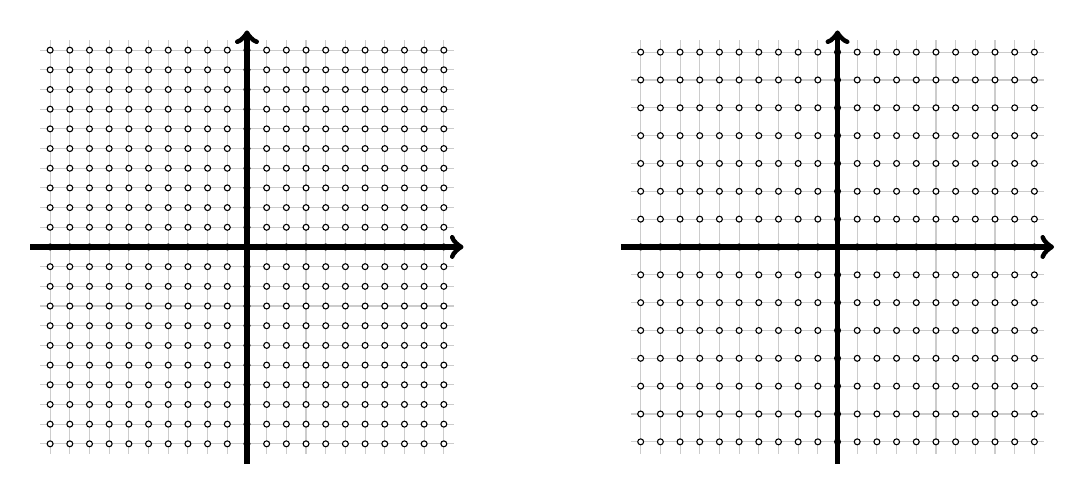
\begin{tikzpicture}[scale=0.25]

\foreach \a in {-10,...,10}{
	\draw[color=black!20!white] (\a,-10.5)--(\a,10.5);
	\draw[color=black!20!white] (-10.5,\a)--(10.5,\a);
}


\foreach \a in {-10,...,10}{
	\foreach \b in {-10,...,10}{
		\draw[fill=white] (\a,\b) circle (0.15);
	}
}

\draw[->, line width=2] (-11,0)--(11,0);
\draw[->, line width=2] (0,-11)--(0,11);

\begin{scope}[xshift=30cm]
\foreach \a in {-10,...,10}{
	\draw[color=black!20!white] (\a,-10.5)--(\a,10.5);
}

\foreach \a in {-7,...,7}{
	\draw[color=black!20!white] (-10.5,1.414*\a)--(10.5,1.414*\a);
}


\foreach \a in {-10,...,10}{
	\foreach \b in {-7,...,7}{
		\draw[fill=white] (\a,\b*1.414) circle (0.15);
	}
}

\draw[->, line width=2] (-11,0)--(11,0);
\draw[->, line width=2] (0,-11)--(0,11);
\end{scope}

\end{tikzpicture} \\ 
The first grid represents $\mathcal{O}_K = \mathbb{Z}[i]$ where $K = \mathbb{Q}(\sqrt{-1}) \simeq \mathbb{Q}[x]/(x^2 + 1)$. \\ \\
The second grid represents $\mathcal{O}_K = \mathbb{Z}[\sqrt{2}]$ where $K = \mathbb{Q}(\sqrt{2}) \simeq \mathbb{Q}[x]/(x^2 - 2)$. \\ \\
Our goal is to strip away these grid to obtain the set of prime numbers in both settings.  These are well-studied problems with detailed algebraic solutions, the goal is to solve these examples for ourselves. \\ \\
In the case of $\mathbb{Z}[i]$ all that seems to matter is the first quadrant.  The group action $\times \sqrt{-1}$ is, for the moment a $90^\circ$ rotation counterclockwise.  We have that $(1) < (1+i) < (2) < (1+2i) $ with nothing in between.  These are \textbf{ideals} and we have $(1+i) = (1-i)$.  We have that $(2)$ is \textbf{not}
prime.  $(2) = (1+i)^2 = (1+i)(1-i)$ \\ \\
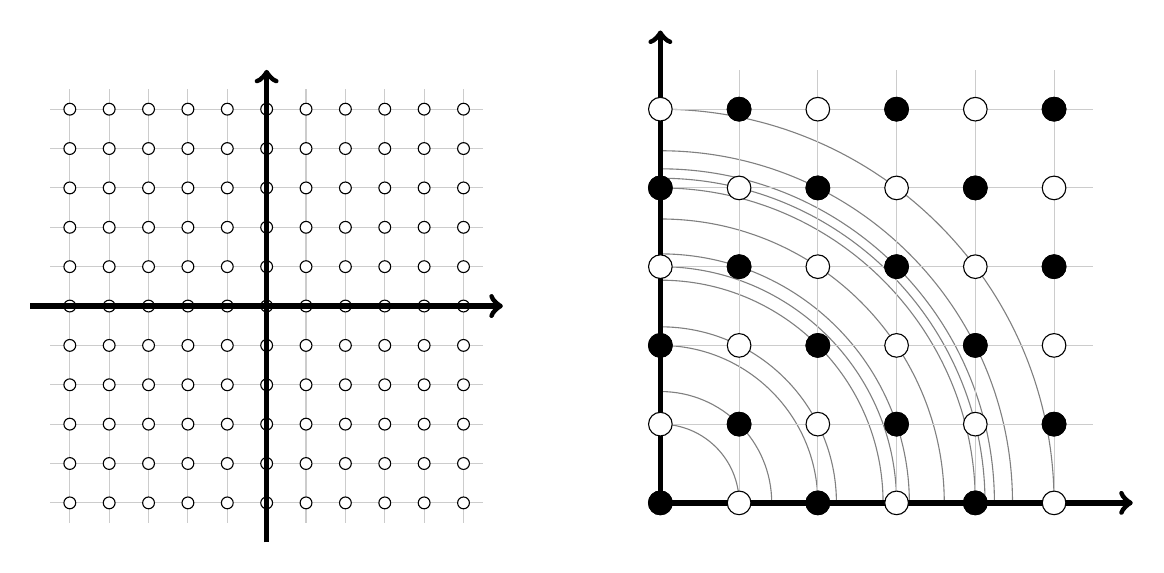
\begin{tikzpicture}[scale=0.5]

\foreach \a in {-5,...,5}{
	\draw[color=black!20!white] (\a,-5.5)--(\a,5.5);
	\draw[color=black!20!white] (-5.5,\a)--(5.5,\a);
}


\foreach \a in {-5,...,5}{
	\foreach \b in {-5,...,5}{
		\draw[fill=white] (\a,\b) circle (0.15);
	}
}

\draw[->, line width=2] (-6,0)--(6,0);
\draw[->, line width=2] (0,-6)--(0,6);


\begin{scope}[xshift=10cm, scale=2, yshift=-2.5cm]

\foreach \r in {  0.        ,   1.        ,   1.41421356,   2.        ,
         2.23606798,   2.82842712,   3.        ,   3.16227766,
         3.60555128,   4.        ,   4.12310563,   4.24264069,
         4.47213595,   5.    }
{

	\draw[color=black!50!white] (\r,0) arc (0:90:\r);

}

\foreach \a in {0,...,5}{
	\draw[color=black!20!white] (\a,0)--(\a,5.5);
	\draw[color=black!20!white] (0,\a)--(5.5,\a);
}

\draw[->, line width=2] (0,0)--(6,0);
\draw[->, line width=2] (0,0)--(0,6);




\foreach \a in {0,...,5}{
	\foreach \b in {0,...,5}{
		\draw[fill=white] (\a,\b) circle (0.15);
	}
}





\draw[fill=black] (0,0) circle (0.15);
\draw[fill=black] (0,2) circle (0.15);
\draw[fill=black] (1,1) circle (0.15);
\draw[fill=black] (2,0) circle (0.15);
\draw[fill=black] (0,4) circle (0.15);
\draw[fill=black] (1,3) circle (0.15);
\draw[fill=black] (2,2) circle (0.15);
\draw[fill=black] (3,1) circle (0.15);
\draw[fill=black] (4,0) circle (0.15);
\draw[fill=black] (1,5) circle (0.15);
\draw[fill=black] (2,4) circle (0.15);
\draw[fill=black] (3,3) circle (0.15);
\draw[fill=black] (4,2) circle (0.15);
\draw[fill=black] (5,1) circle (0.15);
\draw[fill=black] (3,5) circle (0.15);
\draw[fill=black] (4,4) circle (0.15);
\draw[fill=black] (5,3) circle (0.15);
\draw[fill=black] (5,5) circle (0.15);

\end{scope}


\end{tikzpicture}\\
We know that $(1+2i) \big| (5)$ and we even have that $5 = (1+2i)\times(1-2i)$.  At first glance $(3) \approx (1 + 2i)\approx 2 \times (1+i)$. \\
The algebra is slightly misleading here since it makes things that are close together (approximate over $\mathbb{R}$) look very distant.  This could be useful to us. \\\\
\textbf{Ex.} $(1+2i) \stackrel{?}{=} (1-2i)$ \\ \\
The answer is definitely no.  If we join the two ideals together into a single idea, we obtain a notational diaster:
$$2 = (1+2i)+(1-2i) \in (1+2i,1-2i)$$ 
And therefore, $(1+2i) - 2 = 1$ is in this ideal as well.  By something very much like \textbf{Bezout's Theorem} we could obtain two complex integers $a,b \in \mathbb{Z}[i]$ with:
$$a \times (1+2i) + b \times (1-2i)  = 1 \in \mathbb{Z}[i]$$
This is to say the ideasl $(1+2i)$ and $(1-2i)$ are relatiely prime, even if it takes a few manipulations.  
$$ 1 = (1+2i) - 2i = (1+2i) - 2i \times \big( (1+2i)+(1-2i)\big) 
= (1-2i) \times (1+2i) + (-2i)\times (1-2i) $$
The determinant of these four numbers should be exactly $1$.
$$ \left|
\begin{array}{rc} 
1-2i & 1-2i \\
  2i & 1+2i 
\end{array}
 \right| =  
 (1-2i) \times (1+2i) - (2i)\times (1-2i) = 1 $$
There are two prime ideals or ``places" over Gaussian integers.  This is what we mean by ``splitting of primes".  $(5) > (1+2i)$ and $(5) > (1-2i)$.  There are two places over $5$ and $(1+2i) \cap (1-2i) = (1) = \mathbb{Z}[i]$. 

\newpage

\noindent Splitting of primes in $\mathbb{Z}[\sqrt{2}]$ and therefore Pell equations, $x^2 - 2y^2 = p$ are required to evaluate zeta functions such as $\zeta_F(2)$ and $\zeta_F(-1)$.  Whether you count ideals, or use the Euler product a look at the Pell equation is necessary. 
$$ \zeta_F(2) = \sum_\mathfrak{a} \frac{1}{N(\mathfrak{a})^2} = \prod_\mathfrak{p} \frac{1}{1 - \frac{1}{N(\mathfrak{p})^2}}$$
and $\chi$ is a character in the ideal class group. This thing is indexed over ideals $\mathfrak{a}, \mathfrak{p} \subseteq K$.  \\ \\
I don't understand why people don't say ideals are grids in the Euclidean plane.  At this point we are already almost totally reliant of the construct of $\mathbb{Z}$ as a number system.  Just draw a grid and count the grids.  \\ \\
Pell Eq.  The two main strategies I can think of for solving the thing are:
\begin{itemize}
\item factoring immediately: $x^2 - 2y^2 = (x + \sqrt{2}y)(x - \sqrt{2}y) = p$ 
\item geometry of numbers
\item pigeonhole principle
\end{itemize}
Can we do anymore than regurgitate the answer.  All the Math.StackExchange answers are quick shortcuts and not very mindful.  The paper I'm reading says ``\textit{Let $F$ be a totally real field\dots}" and then I'm going to say $\text{SL}_2\big(\mathbb{Z}[\sqrt{2}]\big)\subseteq \text{SL}_2(\mathbb{R})$ and  on and on. \\ \\
If we try to solve Pell equation with a composite number $n = p_1 p_2 \in \mathbb{Z}$ then things over it should factor.  We even have nice formal names for this derivative behavior.  We could find solutions to the simultaneous congruences:
\begin{eqnarray*}
x_1^2 - 2\,y_1^2 &=& 0 \pmod {p_1} \\ 
x_2^2 - 2\,y_2^2 &=& 0 \pmod {p_2} 
\end{eqnarray*} 
and the Chinese Remainder Theorem (using Pigeonhole or Continued Fractions) could merge these two solutions into a single congruence.  What assures us a solution over $\mathbb{Z}$?  There are two solutions $(p,0), (x,y)$ over each of the two places and we could examine:
$$ (p,0)\mathbb{Z} + (x,y) \mathbb{Z} \quad\text{ or }\quad
(p,0)\mathbb{Z}[\sqrt{2}] + (x,y) \mathbb{Z}[\sqrt{2}] $$
and geometry of numbers should tell us a point of mimimum ``radius" exists and the value is exactly $\mathbb{Z}$.  \\ \\
Is that even true? The shape is not even convex.  The shape for $\mathbb{Z}[\sqrt[3]{2}]$ is convex, but this is not.  So know we have to really look over this lowest rung of the Dirichlet Unit Theorem. \\ \\
I guess the counting is as straightforward as they are saying $a_p = 1$ there's only one solution for each prime.  $a_{p^k}\stackrel{?}{=} k+1$ and perhaps  $a_{pq} \stackrel{?}{=} a_p + a_q$.  The numbers are in OEIS A035185 ``the nmber of divisors of $n \equiv  1,7 (8)$ minus the number of divisors $n \equiv 3,5 (8)$".

\begin{verbatim}
1, 1, 0, 1, 0, 0, 2, 1, 1, 0, 
0, 0, 0, 2, 0, 1, 2, 1, 0, 0, 
0, 0, 2, 0, 1, 0, 0, 2, 0, 0, 
2, 1, 0, 2, 0, 1, 0, 0, 0, 0, 
2, 0, 0, 0, 0, 2, 2, 0, 3, 1, 
0, 0, 0, 0, 0, 2, 0, 0, 0, 0, 
0, 2, 2, 1, 0, 0, 0, 2, 0, 0, 
2, 1, 2, 0, 0, 0, 0, 0, 2, 0, 
1, 2, 0, 0, 0, 0, 0, 0, 2, 0, 
\end{verbatim}
I still have my doubts.
\end{document}